% =====================================================================
%  A1 PORTRAIT POSTER (594 x 841 mm)
%  2026 Niels Bohr Quantum Summer School, SDU Odense
%  Built on article + geometry (no poster class needed).
%  Compile:  pdflatex poster.tex   (twice)
%  EDIT THE AUTHOR / AFFILIATION BLOCK BELOW.
% =====================================================================
\documentclass{article}

\usepackage[paperwidth=594mm,paperheight=841mm,
            top=14mm,bottom=10mm,left=16mm,right=16mm]{geometry}
\usepackage{amsmath,amssymb}
\usepackage{graphicx}
\usepackage{multicol}
\usepackage{booktabs}
\usepackage{xcolor}
\usepackage{array}
\usepackage{colortbl}
\usepackage[font=small,labelfont=bf,skip=3pt]{caption}
\usepackage{helvet}
\renewcommand{\familydefault}{\sfdefault}

\graphicspath{{../figures/}}
\pagestyle{empty}
\setlength{\parindent}{0pt}
\setlength{\columnsep}{10mm}
\setlength{\fboxsep}{4mm}

% ---- palette --------------------------------------------------------
\definecolor{nbblue}{HTML}{123B63}
\definecolor{nbaccent}{HTML}{2A78D6}
\definecolor{nbwarm}{HTML}{EB6834}
\definecolor{nbgreen}{HTML}{1BAF7A}
\definecolor{nblight}{HTML}{EDF3FA}
\definecolor{nbgrey}{HTML}{5A5A57}

% ---- type scale (A1 viewing distance ~1.5 m) ------------------------
\newcommand{\titlefont}{\fontsize{58}{68}\selectfont}
\newcommand{\authfont}{\fontsize{28}{34}\selectfont}
\newcommand{\afffont}{\fontsize{21}{26}\selectfont}
\newcommand{\sectfont}{\fontsize{28}{34}\selectfont}
\newcommand{\bodyfont}{\fontsize{19}{23}\selectfont}
\newcommand{\bigfont}{\fontsize{22}{27}\selectfont}
\newcommand{\numfont}{\fontsize{42}{48}\selectfont}
\newcommand{\capfont}{\fontsize{16}{20}\selectfont}

\captionsetup{font={sf,footnotesize}}
\renewcommand{\captionfont}{\capfont\color{nbgrey}}

% ---- building blocks ------------------------------------------------
\newcommand{\headsec}[1]{%
  \par\vspace{3.5mm}%
  \colorbox{nbblue}{\begin{minipage}{\dimexpr\linewidth-2\fboxsep\relax}
    \vspace{1mm}\color{white}\sectfont\textbf{#1}\vspace{1mm}
  \end{minipage}}\par\vspace{3mm}}

\newcommand{\keybox}[2]{%
  \par\vspace{2mm}%
  {\color{#1}\rule{\linewidth}{1.2mm}}\par\vspace{-1mm}
  \colorbox{nblight}{\begin{minipage}{\dimexpr\linewidth-2\fboxsep\relax}
    \vspace{1mm}\bodyfont #2\vspace{1mm}
  \end{minipage}}\par\vspace{2mm}}

% headline number + label
\newcommand{\statnum}[3]{%
  \begin{minipage}[t]{#1}\centering
    {\numfont\color{#2}\textbf{#3}}
  \end{minipage}}

\begin{document}
\bodyfont

% =====================================================================
%  HEADER  --- EDIT AUTHORS AND AFFILIATIONS HERE
% =====================================================================
\begin{center}
\colorbox{nbblue}{%
\begin{minipage}{\dimexpr\linewidth-2\fboxsep\relax}
\centering
\vspace{4mm}
{\color{white}\titlefont\textbf{Data Association for Multiple Hypothesis
Tracking}}\\[2mm]
{\color{white}\titlefont\textbf{on a Neutral-Atom Quantum Computer}}\\[6mm]

% ---------------- AUTHOR SLOTS (replace the four names) -------------
{\color{white}\authfont
Author One\,$^{1}$ \quad\textbullet\quad
Author Two\,$^{2}$ \quad\textbullet\quad
Author Three\,$^{3}$ \quad\textbullet\quad
Author Four\,$^{4}$}\\[4mm]

% ---------------- AFFILIATIONS (replace) ----------------------------
{\color{white}\afffont
$^{1}$Affiliation One, City, Country \quad
$^{2}$Affiliation Two, City, Country \quad
$^{3}$Affiliation Three, City, Country \quad
$^{4}$Affiliation Four, City, Country}\\[3mm]

{\color{nblight}\afffont
2026 Niels Bohr Quantum Summer School \quad$\vert$\quad
University of Southern Denmark, Odense \quad$\vert$\quad
Challenge 7}
\vspace{4mm}
\end{minipage}}
\end{center}

\vspace{4mm}

% ---- headline result strip ------------------------------------------
\colorbox{nblight}{%
\begin{minipage}{\dimexpr\linewidth-2\fboxsep\relax}
\centering\vspace{1mm}
\begin{tabular}{@{}p{95mm}@{\hspace{8mm}}p{95mm}@{\hspace{8mm}}p{95mm}@{\hspace{8mm}}p{95mm}@{\hspace{8mm}}p{95mm}@{}}
\centering{\numfont\color{nbgreen}\textbf{21/21}} &
\centering{\numfont\color{nbgreen}\textbf{19.2}} &
\centering{\numfont\color{nbwarm}\textbf{0.86$\times$}} &
\centering{\numfont\color{nbwarm}\textbf{34\%}} &
\centering{\numfont\color{nbaccent}\textbf{12 / 256}}
\tabularnewline[1mm]
\centering\bodyfont instances solved exactly &
\centering\bodyfont benchmark reproduced &
\centering\bodyfont sampling gain ($<$1 = none) &
\centering\bodyfont shots violating a constraint &
\centering\bodyfont atoms needed / available
\tabularnewline
\end{tabular}
\vspace{2mm}
\end{minipage}}

\vspace{6mm}

% =====================================================================
\begin{multicols}{3}

% ---------------------------------------------------------------- COL 1
\headsec{1. The problem}

A sensor returns, at every time step, a set of \textbf{unlabelled} detections.
Nothing says which object produced which detection, some objects are missed, and
some detections are spurious clutter.

Deciding which detections belong together is \textbf{data association}. Committing
early is dangerous: if two objects cross and their identities swap, the error
propagates forever.

\textbf{Multiple Hypothesis Tracking (MHT)} avoids this by keeping many competing
explanations alive and deferring the decision. The price is combinatorial growth
--- and that is where a quantum computer was proposed to help.

\headsec{2. Tracking $\rightarrow$ graph problem}

Following Papageorgiou \& Salpukas [1], each candidate \textbf{track} becomes a
vertex weighted by its log-likelihood-ratio score, and an edge joins two tracks
that claim the \textbf{same detection} --- one detection cannot come from two
objects.

The best global hypothesis is then a
\textbf{Maximum Weight Independent Set (MWIS)}:
\[
  \max \sum_i w_i x_i
  \qquad\text{s.t.}\qquad
  x_i + x_j \le 1 \ \ \forall (i,j)\in E .
\]

The weight is built recursively from the sensor model,
\[
  \Delta\mathrm{LLR} =
  \begin{cases}
    \log(1-P_D) & \text{missed},\\[3pt]
    \log\dfrac{P_D\,\mathcal{N}(\nu;0,S)}{\beta_{\mathrm{FA}}} & \text{detected},
  \end{cases}
\]
where $\beta_{\mathrm{FA}}$ is the clutter density: in a clean scene a
coincidence means something, in a noisy one it does not.

\keybox{nbaccent}{\textbf{MHT needs more than the best answer.} Track confidence
requires a \emph{population} of hypotheses:
\[
  P\{H_j\}=\frac{e^{L_{H_j}}}{1+\sum_i e^{L_{H_i}}},
  \quad P\{T_i\}=\!\!\!\sum_{j:\,T_i\in H_j}\!\!\! P\{H_j\}.
\]
This is the property the quantum approach was meant to exploit.}

\headsec{3. Why neutral atoms}

Two atoms closer than the \textbf{blockade radius}
\[
  R_b=\left(\frac{C_6}{\hbar\Omega}\right)^{1/6}
\]
cannot both be excited to a Rydberg state. Placing incompatible tracks within
$R_b$ enforces $x_i+x_j\le1$ \textbf{in hardware}, with no penalty term to tune:
\[
  H/\hbar=-\sum_i\delta_i n_i+\sum_{i<j}\frac{C_6}{r_{ij}^{6}}n_i n_j .
\]

Track scores become \textbf{local detunings} via the Detuning Map Modulator.
It only shifts downwards, so $m_i=1-w_i/w_{\max}$ gives
$\delta_i=\delta_{\max}w_i/w_{\max}$ --- needing $w_i>0$, which the
``positive-score tracks only'' rule supplies for free.

% ---------------------------------------------------------------- COL 2
\headsec{4. Pipeline}

\textbf{Classical:} Kalman prediction $\rightarrow$ gating $\rightarrow$ track
branching $\rightarrow$ LLR scoring $\rightarrow$ pruning, merging, $N$-scan
pruning $\rightarrow$ clustering into independent sub-problems.

\textbf{Quantum, per cluster:} geometric embedding $\rightarrow$ optical-tweezer
register $\rightarrow$ adiabatic sweep $\rightarrow$ measure $\rightarrow$ repeat.

\keybox{nbgreen}{\textbf{Classical pruning is what makes it fit.} The largest
cluster over a whole scenario was \textbf{9 vertices} --- far inside a 256-atom
device. Gating, confirmation, track merging and $N$-scan pruning, \emph{not} the
quantum step, keep the problem small. Drop track merging and clusters inflate
into near-cliques no planar register can hold.}


\columnbreak

\headsec{5. The geometric embedding}

On hardware you do \textbf{not} choose the edges --- physics decides them from
distance. The graph solved is always a \textbf{unit-disk graph}; an MHT graph is
not. We need
\[
  \|p_i-p_j\|<R_b \ \text{(edge)},\qquad
  \|p_i-p_j\|>R_b \ \text{(non-edge)},
\]
solved by penalty minimisation with random restarts, in units of $R_b$.

\textbf{$\Omega$ is derived, not chosen.} The layout fixes only distance
\emph{ratios}. A larger $R_b$ gives atoms room but costs Rabi frequency as
$R_b^{-6}$, and too small an $\Omega$ never leaves the ground state inside the
device's 6\,$\mu$s limit.

\begin{center}
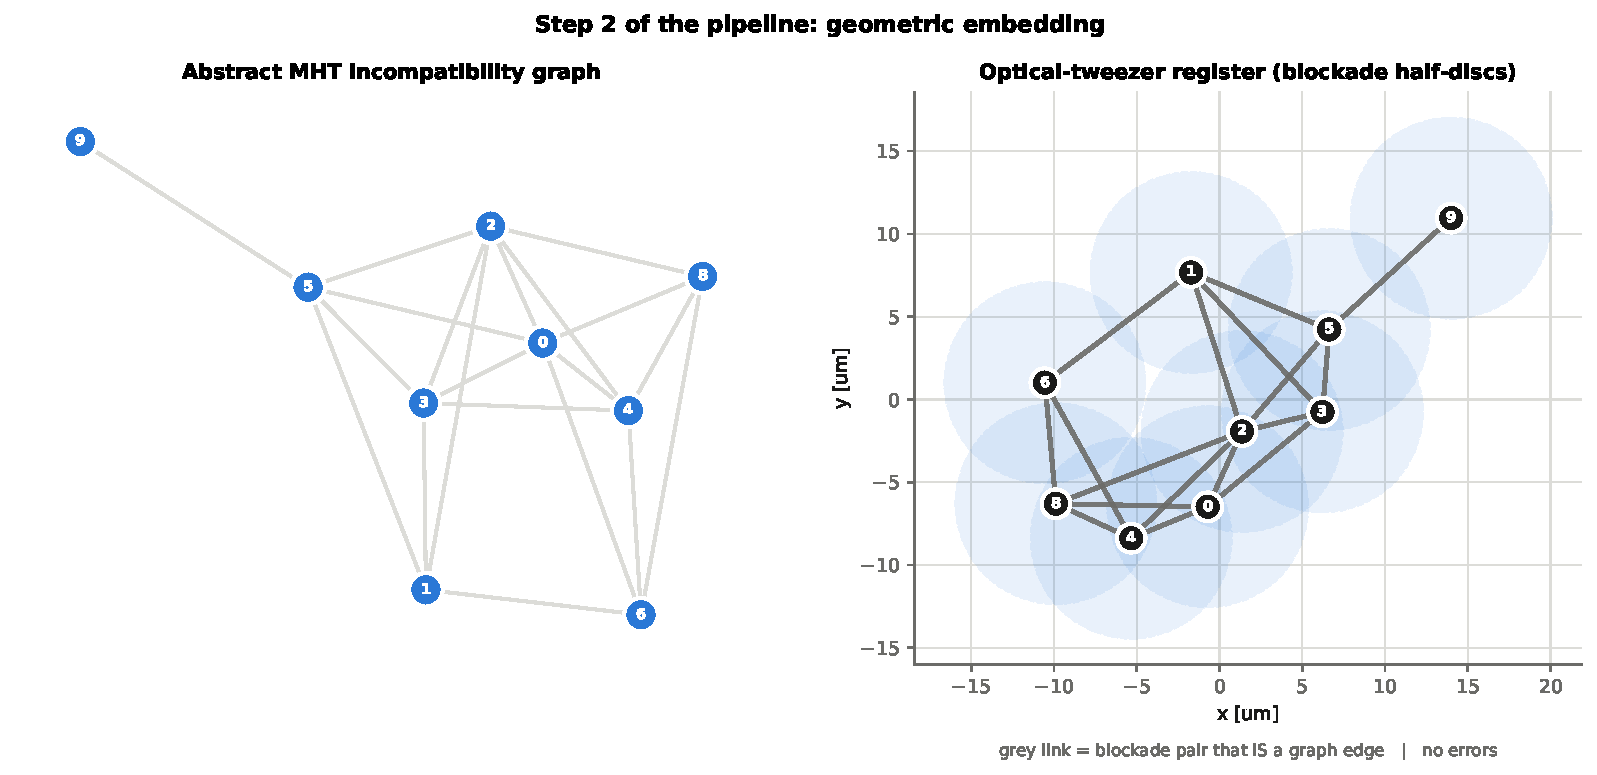
\includegraphics[width=0.96\linewidth]{embedding.pdf}
\captionof{figure}{A real MWIS instance from the tracker: abstract conflict
graph (left) and the atom register realising it (right). Shaded discs show
blockade range.}
\end{center}

\keybox{nbwarm}{\textbf{Cliques are the obstruction.} A $k$-clique needs $k$
atoms pairwise \emph{within} $R_b$ yet pairwise $\ge 5\,\mu$m apart. Feasibility
depends only on $\rho=R_b/d_{\min}\approx2.4$: a hexagon plus centre gives 7
points at ratio exactly 2, so $\ge7$ fit; the limit is $\approx9$. Each track
family \emph{is} a clique --- so capping branches per family is a hardware
constraint, not a tuning choice.}

\headsec{6. Validation}

We reproduce the worked example of [1] --- six tracks with published
incompatibility lists; optimum $\{3,6\}$, weight \textbf{19.2}. Classical solver
and atom array both return exactly this, the array sampling it in
\textbf{93--95\%} of shots with a defect-free embedding.

In closed-loop tracking on synthetic radar (5 converging targets, $P_D=0.9$,
Poisson clutter) the array solved \textbf{21 instances and matched the exact
optimum on all 21}, following every object with 100\% association accuracy.

% ---------------------------------------------------------------- COL 3
\headsec{7. Testing the advantage}

Optimisation alone proves nothing here --- classical solvers find the optimum
instantly at $n\le12$. The real claim concerns $P\{H_j\}$: the array should give
a \emph{distribution} at fixed cost, while classical enumeration cost grows with
how many hypotheses exist (up to $3^{n/3}$).

\textbf{Real data.} \texttt{PhC-C2DL-PSC}, Cell Tracking Challenge [2]: 300
frames of phase-contrast microscopy, cells proliferating $74\rightarrow661$.
Detections from raw pixels (recall $\approx0.5$, precision $\approx0.85$); ground
truth grades the detector only. Six MWIS instances of 9--12 tracks.

\textbf{Metric: posterior mass per sample.} Counting hypotheses would rate a
0.1\% explanation equal to one carrying 90\%. A ``sample'' $=$ one measure cycle
/ annealing run / construction; identical post-processing for all.

\vspace{2mm}
{\bigfont
\begin{tabular}{@{}l r r@{}}
\toprule
\textbf{Sampler} & \textbf{Samples} & \textbf{Prec.}\\
\midrule
Simulated annealing      & \textbf{23.6} & 98.0\%\\
\rowcolor{nblight} Neutral atoms      & 27.5 & 97.8\%\\
Randomised greedy        & 35.3 & 91.0\%\\
Atoms, no repair         & 32.2 & 64.2\%\\
\bottomrule
\end{tabular}}
\vspace{1mm}
\captionof{table}{Samples to capture 90\% of the posterior mass.}

\columnbreak

\begin{center}
% panel 1 of route1_curves.pdf, cropped so it is legible at A1 print size
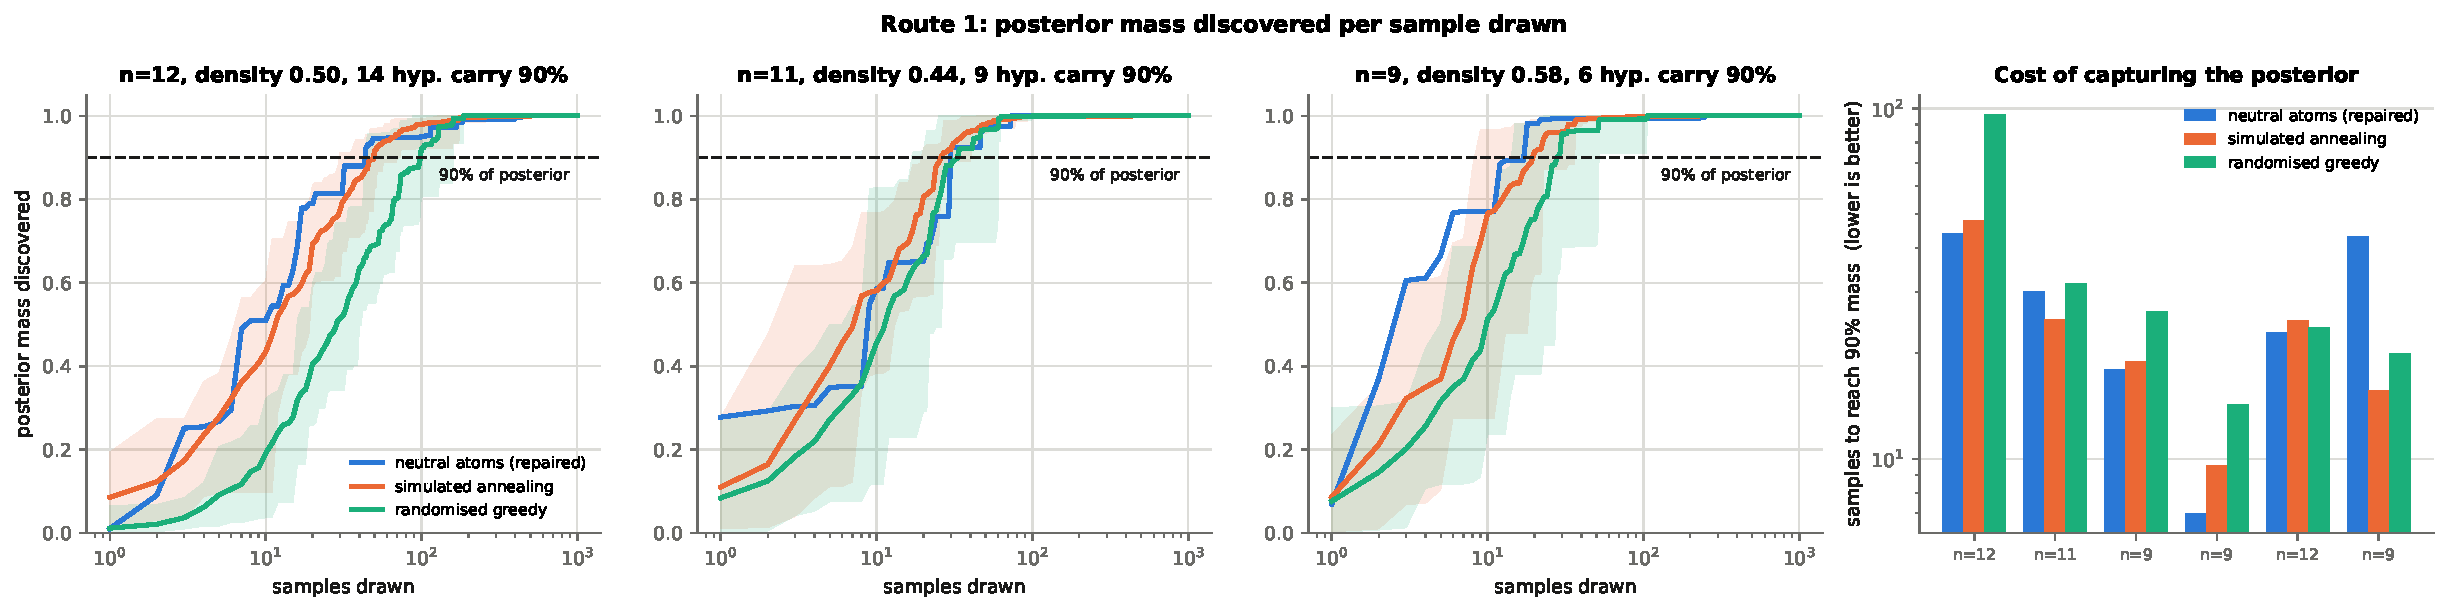
\includegraphics[width=0.80\linewidth,trim={0 0 875 0},clip]{route1_curves.pdf}
\captionof{figure}{Posterior mass discovered against samples drawn, for one
instance. Shading spans repeats of the classical samplers.}
\end{center}

\keybox{nbwarm}{\textbf{The claim is not supported.} The array needed
\emph{more} samples than annealing. The margin is small --- it won on 4 of 6
instances and beat randomised greedy clearly --- so the honest reading is
``indistinguishable at this sample size'', not a clear loss. Six instances
cannot settle it either way.}

\headsec{8. Why}

\textbf{Embeddability dominates.} Real conflict graphs had mean density
\textbf{0.66}, and \textbf{34\%} of shots violated an edge. The blockade --- the
one mechanism meant to enforce constraints for free --- was not enforcing them.
Classical repair then does that work, and a repaired shot is no longer a physical
sample.

\begin{center}
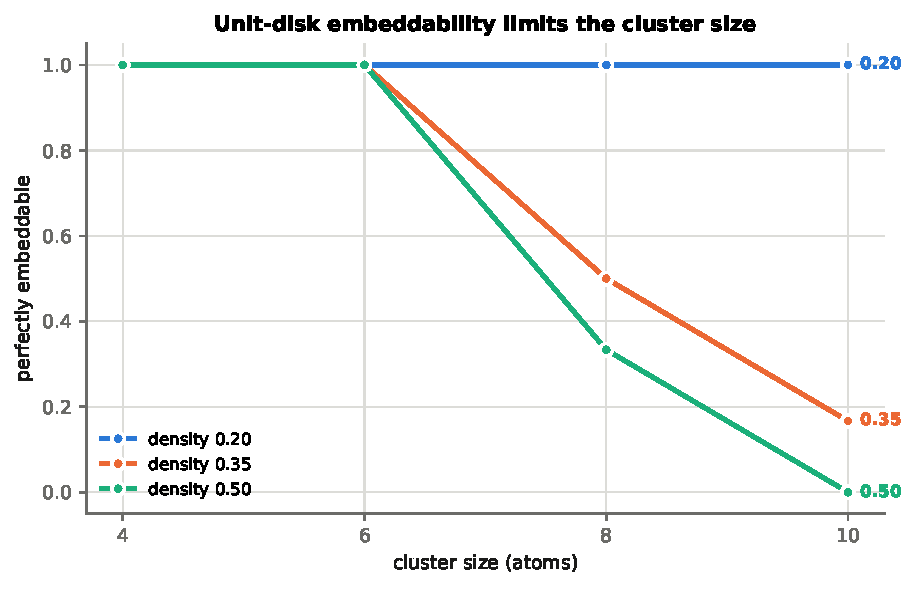
\includegraphics[width=0.82\linewidth]{embeddability.pdf}
\captionof{figure}{Perfect unit-disk embeddings vanish with size and density.
The limit is geometry, not qubit count.}
\end{center}

\textbf{Concentration fights coverage.} Capturing 90\% of the posterior needs
$\approx7$ distinct hypotheses, but an adiabatic sweep returns \emph{one}. Sweep
duration moves $P(\text{optimum})$ from 8\% to 99\% while diversity moves the
other way --- a knob with no classical analogue, but not enough to close the gap.


\headsec{9. Conclusions}

\begin{itemize}\setlength\itemsep{2mm}
\item The physics mapping is sound; the implementation reproduces published
      results exactly.
\item \textbf{$\lambda$ is not free.} The penalty is $C_6/r_{ij}^6$, set by
      atom placement. You choose $\delta_{\max}/\Omega$, bounded on \emph{both}
      sides; measured window $2\lesssim\delta_{\max}/\Omega\lesssim5.6$.
\item \textbf{Geometry binds, not qubit count.} We never needed more than 12 of
      256 atoms.
\item \textbf{Weights are quantised:} score differences below $\approx2.6$ LLR
      are invisible to the hardware.
\end{itemize}

\keybox{nbaccent}{\textbf{Consequence.} Making the graph \emph{natively}
unit-disk is a \textbf{precondition}, not a refinement. Untested and promising:
place atoms by proximity in \emph{track state space}, where tracks sharing a
detection are already close.}

\textbf{Open:} repair bias; unresolved targets (two objects merging into one
detection \emph{should} share it); hardware noise, which hits the weight encoding
directly since the weights \emph{are} detunings.

\vspace{3mm}
{\capfont
\textbf{Refs.} [1] Papageorgiou \& Salpukas, Springer 2009, 235--255.
[2] Ulman et al., \emph{Nat.\ Methods} \textbf{14}, 1141 (2017),
celltrackingchallenge.net. [3] Silv\'erio et al., \emph{Quantum} \textbf{6}, 629
(2022). [4] Ebadi et al., \emph{Science} \textbf{376}, 1209 (2022).
\quad\textbf{Code:} \texttt{code/}, Pulser/QuTiP emulator.}

\end{multicols}
\end{document}
